% ──────────────────────────────────────────────────────────────────────────────
% EXPERIMENTS AND RESULTS SECTION DRAFT
% ──────────────────────────────────────────────────────────────────────────────

\section{Experiments and Results}
\label{sec:experiments}

The experiments are structured as follows.
The first compares the proposed RL framework against three baselines across
three datasets and two bias conditions, establishing the main fairness-utility
tradeoff results.
The second examines how each method's fairness degrades as positive-class
scarcity increases, motivating the specific problem regime targeted by this
work.
The third through sixth are ablation studies that isolate the contribution of
individual design choices: PCA compression of the action space, beta classifier
training duration, delta action scale, and two-phase generation.

All experiments use a common evaluation protocol of five seeds per
configuration, reporting mean $\pm$ standard deviation.
Three datasets are evaluated: \textit{Census Income} (sex and race as protected
attributes; primary fairness dataset), \textit{Credit Card Default} (sex as
protected attribute; secondary dataset), and \textit{HAR} (physical activity
recognition; included as a third dataset per funding requirements).
Bias is injected by downsampling positive-class examples from the disadvantaged
group to a target retention rate $p_+$; two conditions are tested across all
datasets: $p_+ = 10\%$ (high scarcity) and no-bias (natural class proportions).
Fairness is measured by Equal Opportunity gap (EO, $\downarrow$) and
Demographic Parity gap (DP, $\downarrow$); utility by AUC ($\uparrow$) and
accuracy ($\uparrow$).
The combined Fairness-Utility Score $\text{FUS} = (1 - \text{EO}) \times
\text{AUC}$ summarises the tradeoff in a single scalar ($\uparrow$).
Three baselines are included: Group DRO~\cite{sagawa2020groupdro},
OT Repair~\cite{black2020repair}, and CT-GAN~\cite{xu2019ctgan}.
A no-intervention baseline — a classifier trained on biased real data without
any augmentation — is also reported to establish the upper bound on EO before
any method is applied.

\subsection{Main Comparison}
\label{sec:results:main}

Tables~\ref{tab:nobias_compressed} and~\ref{tab:010_compressed} report the
fairness-utility tradeoff for all methods under the no-bias and
$p_+ = 10\%$ conditions; Figure~\ref{fig:tradeoff_all} shows the same
results as a scatter plot.
This experiment is included to assess whether the proposed framework achieves a
competitive tradeoff between fairness and predictive utility relative to
established reweighting and generative baselines under both data conditions.

\paragraph{Census (bias = 10\%).}
Under high positive-class scarcity the RL framework achieves the lowest EO of
all methods, more than $4\times$ lower than Group DRO and OT Repair, while
also recording the highest accuracy.
CT-GAN shows substantially higher variance across seeds.
The RL framework achieves the highest FUS, indicating the fairness gain is
not offset by a loss in predictive utility.

\paragraph{Census (no bias).}
When the training data are unbiased the RL framework remains competitive,
finishing behind Group DRO in EO but ahead of CT-GAN and OT Repair.
The result confirms that the framework does not degrade when applied to
unbiased data.

\paragraph{Credit card (bias = 10\%).}
On the credit dataset the no-intervention alpha model already achieves a low
EO gap, leaving limited room for improvement across all methods; differences
between methods are within the margin of uncertainty.
OT Repair records the lowest EO; the RL framework is competitive on accuracy
but lower on AUC.

\paragraph{Credit card (no bias).}
Under no-bias conditions all methods are near-parity on both fairness and
utility metrics.

% ── Figure reference ──
\begin{figure}[t]
    \centering
    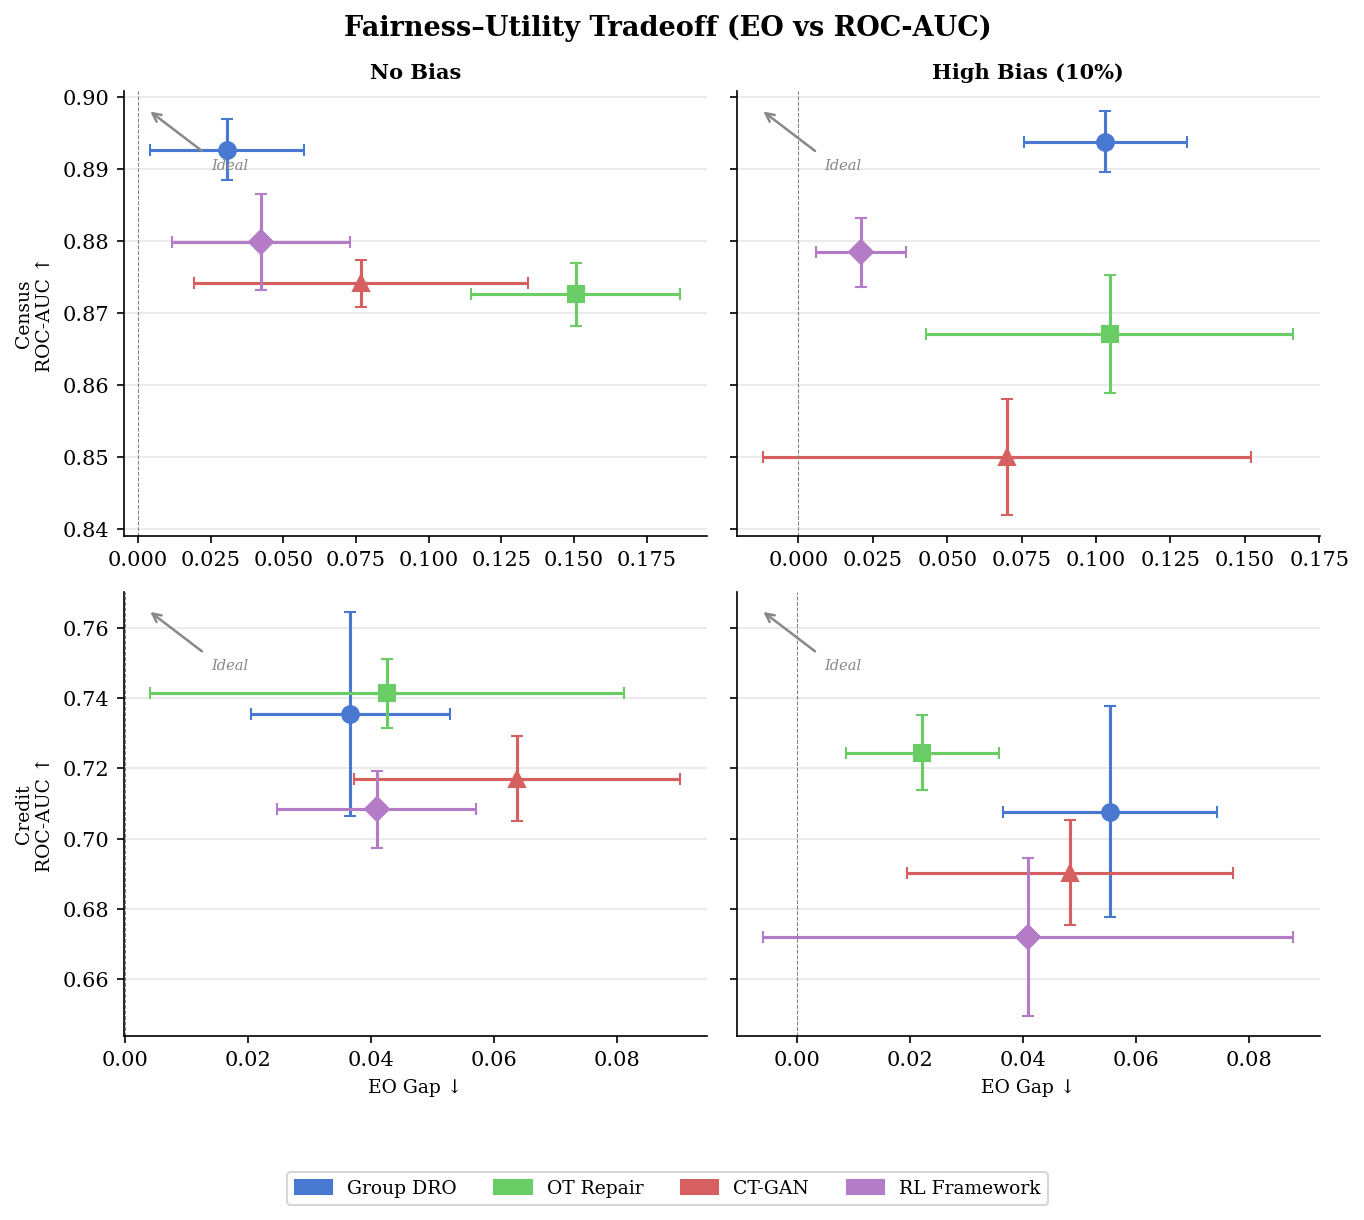
\includegraphics[width=\linewidth]{paper_figures/fig_tradeoff_all.png}
    \caption{Fairness-utility tradeoff (EO gap vs AUC) across methods and
    datasets. Error bars show $\pm 1$ s.d.\ over 5 seeds. The ideal direction
    (lower EO, higher AUC) is marked.}
    \label{fig:tradeoff_all}
\end{figure}

\subsection{Effect of Positive-Class Scarcity}
\label{sec:results:bias_level}

This experiment evaluates how each method responds as the degree of
positive-class scarcity is varied, which is the defining characteristic of
the problem regime this work addresses.
Figure~\ref{fig:eo_vs_bias} plots mean EO gap against bias severity for each
method on both datasets.
On Census, Group DRO and OT Repair show steep EO degradation as $p_+$ drops
from the natural rate (${\sim}24\%$) to $10\%$: Group DRO rises from
$0.031$ to $0.103$, OT Repair from $0.151$ to $0.105$.
The RL framework's EO moves from $0.042$ to $0.021$ across the same range.
CT-GAN shows a comparable trend to the RL framework but with substantially
higher variance at $10\%$ bias ($\pm 0.082$).
On Credit the scarcity effect is mild across all methods, consistent with the
low alpha-EO baseline on that dataset.

\begin{figure}[t]
    \centering
    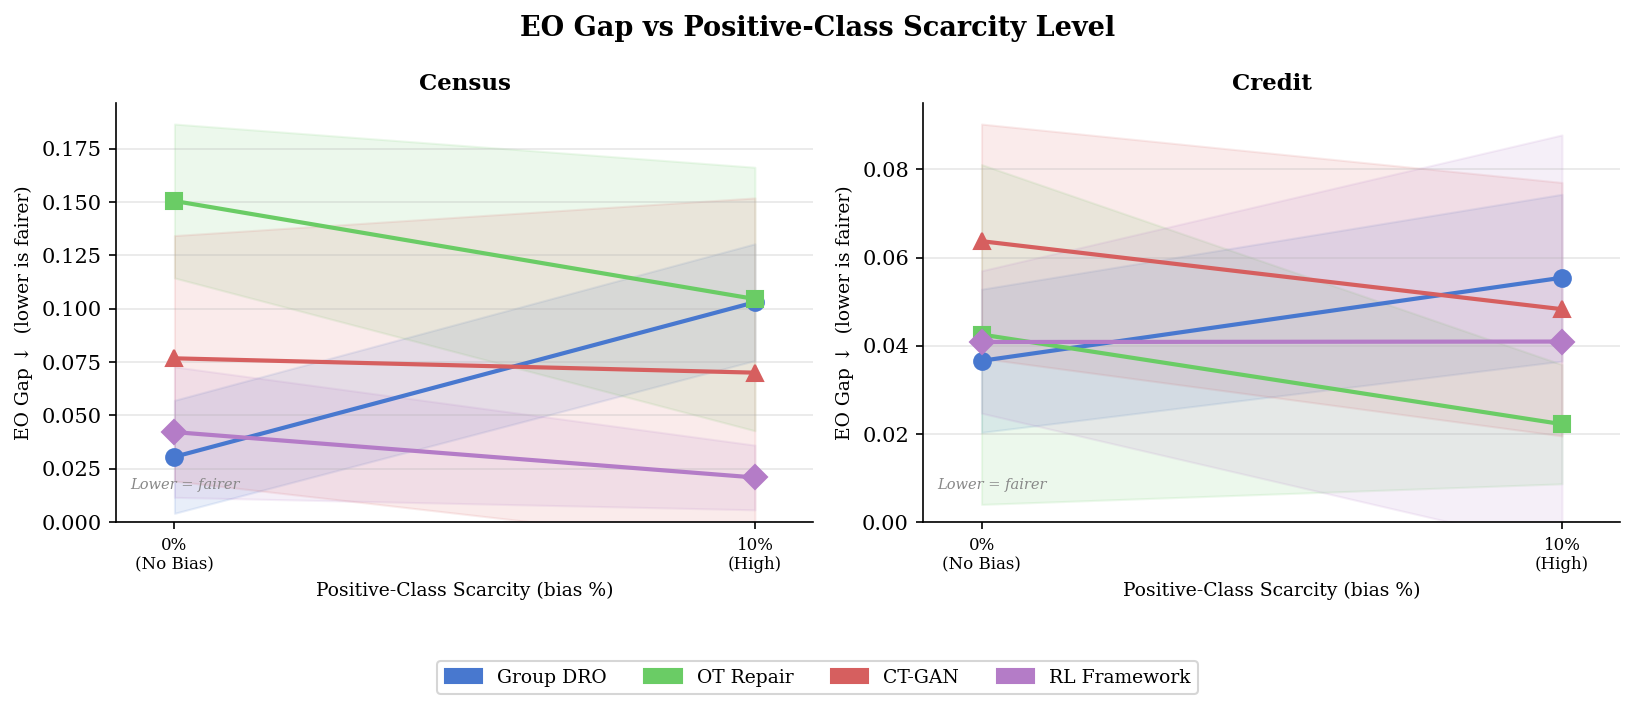
\includegraphics[width=\linewidth]{paper_figures/fig_eo_vs_bias.png}
    \caption{EO gap as a function of positive-class scarcity level (Census and
    Credit). Shaded bands show $\pm 1$ s.d.}
    \label{fig:eo_vs_bias}
\end{figure}

\subsection{Ablation Studies}
\label{sec:results:ablations}

All ablations are performed on the Census dataset at bias $= 10\%$ unless
otherwise noted, using the same 5-seed protocol as the main results.
The default configuration uses PCA compression to 10 components, bounded delta
actions with $\delta = 0.10$, and a 20-epoch beta classifier.

\subsubsection{PCA Compression of the Action Space}
\label{sec:ablation:pca}

This ablation examines whether compressing the agent's action space via PCA
is necessary for effective policy learning.
Without PCA ($= 1$ component), EO rises to $0.111 \pm 0.078$ under the global
reward and $0.089 \pm 0.106$ under the DVRL-weighted reward.
With compression to 10 components, EO falls to $0.021 \pm 0.015$ — a
$5\times$ reduction — demonstrating that dimensionality reduction is a
critical component of the framework.

\subsubsection{Beta Classifier Training Duration}
\label{sec:ablation:epochs}

The beta classifier is retrained from scratch each episode; this ablation
tests how sensitive the reward signal is to the number of training epochs.
Figure~\ref{fig:ffnn_ablation} shows results for 5, 20, and 50 epochs.
At 5 epochs EO is $0.045 \pm 0.046$; at 50 epochs EO rises to
$0.036 \pm 0.018$.
The default of 20 epochs achieves the best EO ($0.021 \pm 0.015$) and the
highest AUC ($0.878 \pm 0.005$).

\begin{figure}[t]
    \centering
    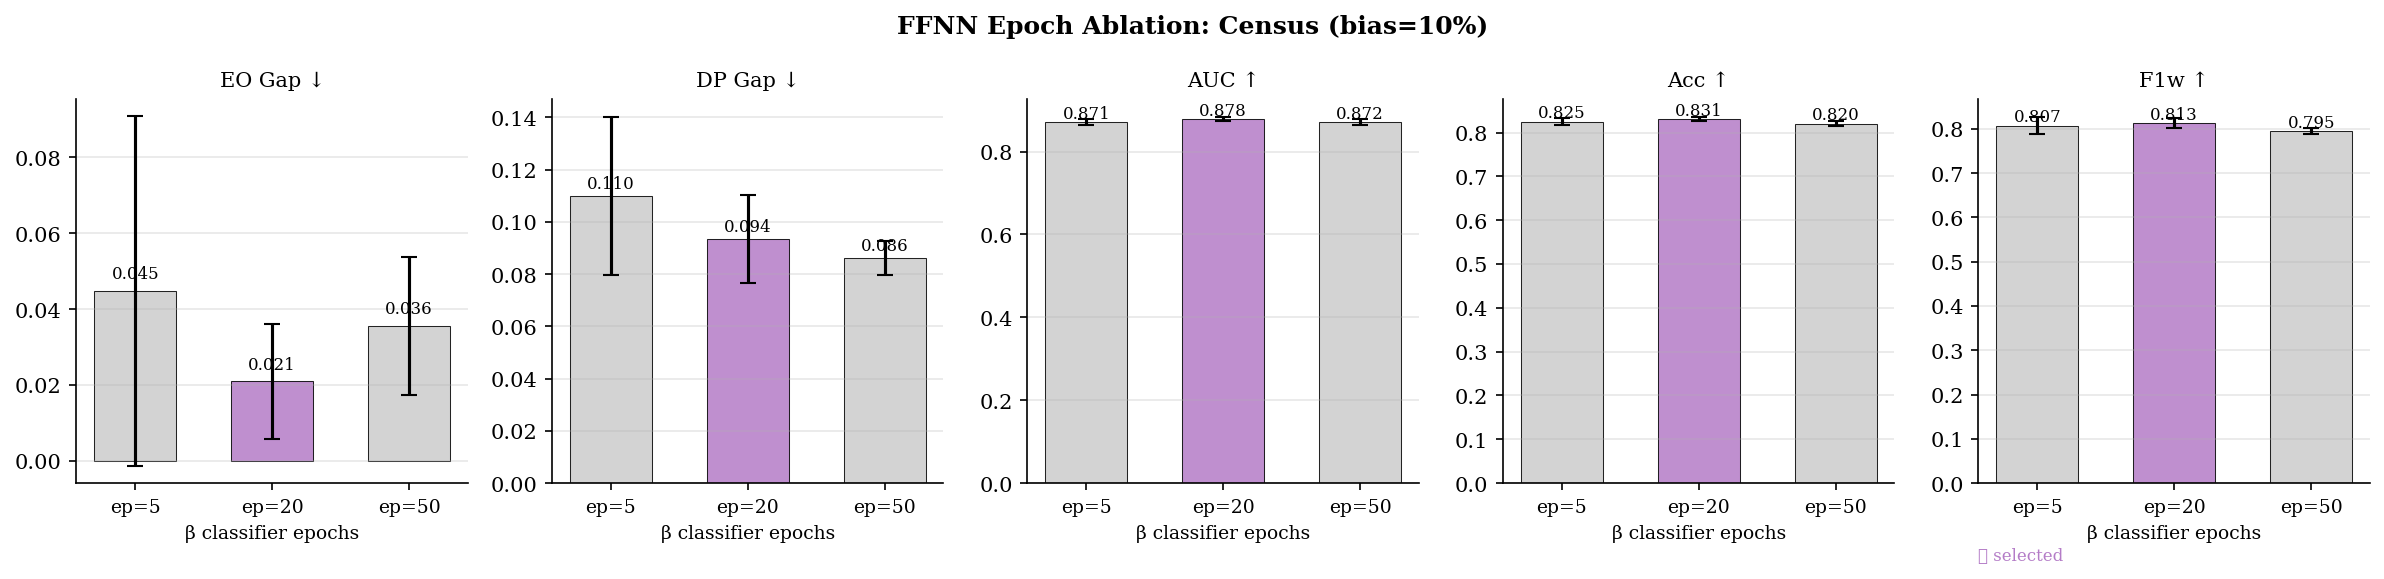
\includegraphics[width=0.9\linewidth]{paper_figures/fig_ffnn_ablation_census.png}
    \caption{Effect of beta classifier training duration (Census, bias $=10\%$,
    5 seeds). The default 20 epochs (highlighted) achieves the best EO and AUC
    across the sweep.}
    \label{fig:ffnn_ablation}
\end{figure}

\subsubsection{Delta Action Scale}
\label{sec:ablation:delta}

This ablation varies the bound $\delta$ on each per-step PCA-space
perturbation to determine the sensitivity of the framework to this
hyperparameter.
At $\delta = 0.05$, EO is $0.085 \pm 0.086$; at $\delta = 0.20$, EO is
$0.083 \pm 0.053$; the default $\delta = 0.10$ produces EO $= 0.021 \pm
0.015$.
Both deviations raise EO by a factor of approximately $4\times$ relative to
the default.

\subsubsection{Two-Phase Generation}
\label{sec:ablation:phase2}

The default framework generates synthetic minority-class (positive) samples
only (Phase 1).
This experiment evaluates a two-phase variant that additionally trains the
agent to generate majority-class (negative) synthetic samples in a second
pass (Phase 1 + Phase 2), assessing whether augmenting both classes provides
further benefit.
Compared to Phase 1 alone (EO $= 0.070 \pm 0.052$, F1$_w = 0.798 \pm
0.015$), Phase 1+2 reduces EO to $0.052 \pm 0.046$ and improves F1$_w$ to
$0.808 \pm 0.006$, with tighter variance across seeds.
Note that these runs use a slightly different configuration (lambda $= [1.0,
1.0]$, global reward only) than the main results; the comparison is
directional rather than a controlled contrast to the headline numbers.

\end{document}
